% Copyright 2004 by Till Tantau <tantau@users.sourceforge.net>.
%
% In principle, this file can be redistributed and/or modified under
% the terms of the GNU Public License, version 2.
%
% However, this file is supposed to be a template to be modified
% for your own needs. For this reason, if you use this file as a
% template and not specifically distribute it as part of a another
% package/program, I grant the extra permission to freely copy and
% modify this file as you see fit and even to delete this copyright
% notice. 
\UseRawInputEncoding
\documentclass{beamer}

% There are many different themes available for Beamer. A comprehensive
% list with examples is given here:
% http://deic.uab.es/~iblanes/beamer_gallery/index_by_theme.html
% You can uncomment the themes below if you would like to use a different
% one:
%\usetheme{AnnArbor}
%\usetheme{Antibes}
%\usetheme{Bergen}
%\usetheme{Berkeley}
%\usetheme{Berlin}
%\usetheme{Boadilla}
%\usetheme{boxes}
%\usetheme{CambridgeUS}
%\usetheme{Copenhagen}
%\usetheme{Darmstadt}
%\usetheme{default}
%\usetheme{Frankfurt}
%\usetheme{Goettingen}
%\usetheme{Hannover}
%\usetheme{Ilmenau}
%\usetheme{JuanLesPins}
%\usetheme{Luebeck}
\usetheme{Madrid}
%\usetheme{Malmoe}
%\usetheme{Marburg}
%\usetheme{Montpellier}
%\usetheme{PaloAlto}
%\usetheme{Pittsburgh}
%\usetheme{Rochester}
%\usetheme{Singapore}
%\usetheme{Szeged}
%\usetheme{Warsaw}

\usepackage{pgfgantt}
%\usepackage{todonotes}
\usepackage{media9}
\usepackage{subfigure}

% Customize Warsaw color 
\setbeamercolor*{palette primary}{use=structure,fg=white,bg=blue!50!black}
\setbeamercolor*{palette secondary}{use=structure,fg=white,bg=blue!60!black}
\setbeamercolor*{palette tertiary}{use=structure,fg=white,bg=blue!70!black}

% Customize Warsaw block title and background colors
\setbeamercolor{block title}{bg=red!50!black,fg=white}

\setbeamertemplate{bibliography item}{\insertbiblabel}  % insert bibliography numbers instead of symbol
\setbeamertemplate{caption}[numbered] % adds the figure or table number to the caption.



\title[System Level Requirements]{Development of Building Energy Management Platform}

% % A subtitle is optional and this may be deleted
% \subtitle{Product Proposal}

\author[B.~Lauer, E.~Watkins]{Brian~Lauer \and Elliot~Watkins \and
Advisor: Dr. Suruz Miah}
% - Give the names in the same order as the appear in the paper.
% - Use the \inst{?} command only if the authors have different
%   affiliation.

\institute[Bradley University] % (optional, but mostly needed)
{
  Department of Electrical and Computer Engineering\\
  Bradley University\\
  1501 W. Bradley Avenue\\
  Peoria, IL, 61625, USA
}
% - Use the \inst command only if there are several affiliations.
% - Keep it simple, no one is interested in your street address.

%\date[November~27,~2018]{Tuesday, November~27,~2018}
\date[October~19,~2020]{Thursday, October~19,~2020}
%\date[December~4,~2018]{Tuesday, December~4,~2016}

% - Either use conference name or its abbreviation.
% - Not really informative to the audience, more for people (including
%   yourself) who are reading the slides online

\logo{\hfill\href{http://www.bradley.edu}{\includegraphics[width=0.75cm]{figs/logoBU1-Print}}}  % place logo in every page 

\subject{Building Energy Management}
% This is only inserted into the PDF information catalog. Can be left
% out. 

% If you have a file called "university-logo-filename.xxx", where xxx
% is a graphic format that can be processed by latex or pdflatex,
% resp., then you can add a logo as follows:

% \pgfdeclareimage[height=0.5cm]{university-logo}{university-logo-filename}
% \logo{\pgfuseimage{university-logo}}

% Delete this, if you do not want the table of contents to pop up at
% the beginning of each subsection:
\AtBeginSubsection[]
{
  \begin{frame}<beamer>{Outline}
    \tableofcontents[currentsection,currentsubsection]
  \end{frame}
}

% Let's get started
\begin{document}

\begin{frame}
  \titlepage
\end{frame}

\begin{frame}{Outline} %
  \tableofcontents%[pausesections]
  % You might wish to add the option [pausesections]
\end{frame}

% Section and subsections will appear in the presentation overview
% and table of contents.
\section{Introduction}
%\section{Project Description}
\section{System Architecture}
\section{High Level Functionality}
\section{Modes of Operation}
\section{End-Use Requirements}

\begin{frame}{Introduction}{} %Elliot
    % Applications of Building Energy Management
    \begin{itemize}
        \item Why BEMS?
            \begin{itemize}
                \item Can help save on energy costs
                \item Less impact on environment
            \end{itemize}
        \item How can the IoT help?
            \begin{itemize}
                \item WiFi integrated into most buildings
                \item Our Web-based approach simplifies development and end-user experience
            \end{itemize}
        \item Overall Goal
            \begin{itemize}
                \item Create a platform in which users can login and access devices connected to a building’s energy supply
                \item Allow the user to closely monitor energy usage throughout a commercial or residential building.
            \end{itemize}
    \end{itemize}
\end{frame}

\begin{frame}{Introduction}{}
\centering
Play Video
\end{frame}

% System Architecture Diagram
\begin{frame}{System Architecture}{} %Elliot
    % High-Level Architecture Figure
    \begin{figure}
        \centering
        \includegraphics[scale=0.4]{figs/highLevelArchitecture.pdf}
        \caption{High level architecture}
        \label{fig:my_label}
    \end{figure}
\end{frame}

% System Architecture - Supported Devices
\begin{frame}{System Architecture - Supported Devices}{} %Elliot
    % What are we using to build this?
    \begin{itemize}
        \item WeMo Switch
            \begin{itemize}
                \item Turn on and off from web server
                \item Record power usage month to month
                \item Plot power usage for a given time frame using MatPlotLib library in Python
            \end{itemize}
        \item Embedded Computer
            \begin{itemize}
                \item Connect to BeagleBone Blue
                \item Control motor drivers from web server
            \end{itemize}
        \item Smart Meter
            \begin{itemize}
                \item Cannot physically implement this
                \item MATLAB has ability to simulate power meters
            \end{itemize}
    \end{itemize}
\end{frame}

\begin{frame}{System Architecture}{}
    \begin{figure}
        \centering
        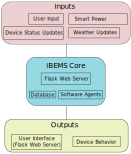
\includegraphics[scale=0.4]{figs/functionalBlockDiagram.pdf}
        \caption{Functional block diagram of the BEMS}
        \label{fig:my_label}
    \end{figure}
\end{frame}

% System Architecture - Inputs
\begin{frame}{System Architecture - Inputs}{} %Elliot
    \begin{itemize}
        \item Users will adjust the operation of a device (turn up temperature of AC unit or turn on/off a light)
        \item Smart Power meters (BEMS core will need to receive power data from MATLAB scripts) will provide real-time power consumption for the entire building
        \item Connected devices will give status updates when prompted by the BEMS Core
        \item The BEMS core will scan a weather service website to receive updates on severe weather that may impact power transmission
    \end{itemize}
\end{frame}


% System Architecture - Web Server
\begin{frame}{System Architecture - BEMS Core}{} %Brian
    % What are we using to build this?
    \begin{itemize}
        \item Python and Javascript
            \begin{itemize}
                \item Python is used to control devices on the back end
                \item Javascript is used to run the web page (user interface)
            \end{itemize}
        \item Flask Web Framework
            \begin{itemize}
                \item Handles rendering device metadata and time-series data to the web page
                \item Routes URLs to view functions
            \end{itemize}
        \item Apache Cassandra and SQLite databases
            \begin{itemize}
                \item Apache Cassandra is a NoSQL database management system for storing time-series device data
                \item SQLite is a simple relational database management system that will be used to store device metadata
            \end{itemize}
        \item Bootstrap and JQuery
            \begin{itemize}
                \item Bootstrap is a CSS framework for creating modern web pages
                \item JQuery is a Javascript library to help with DOM traversal, event handling, and AJAX requests
            \end{itemize}
    \end{itemize}
\end{frame}

\begin{frame}{System Architecture - Outputs}{}
\begin{itemize}
    \item BEMS core will output all data from connected devices to be accessed through the web server via a browser (accessed by any device that can browse the web)
    \item All available data on any smart device will be able to be perused via the platform
\end{itemize}    
\end{frame}

\begin{frame}{Modes of Operation}{}
    \begin{itemize}
        \item \textbf{Mode \#0: Device discovery mode}: networked IoT devices will be automatically discovered on the local building network
        \item \textbf{Mode \#1: Manual device control mode}: the state of each active device will be controllable through an easy-to-use web interface and command line application
        \item \textbf{Mode \#2: Power reporting mode}: a page will be available for reporting overall building power consumption and individual device power consumption
    \end{itemize}
\end{frame}

\begin{frame}{End-Use Requirements}{}
    \begin{itemize}
        \item Device behavior should be implemented to seamlessly support different status configurations
        \item Users (building admins, employees, home owners) will have the ability to see a plot of the past energy usage of a device 
        \item Python's Matplotlib package will form the basis for the plotting functionality 
        \item Support for new devices should be easily developed through multiple layers of abstractions
    \end{itemize}    
\end{frame}

% You can reveal the parts of a slide one at a time
% with the \pause command:
%\begin{frame}{Second Slide Title}
%  \begin{itemize}
%  \item {
%    First item.
%    \pause % The slide will pause after showing the first item
%  }
  %\item {   
  %  Second item.
 % }
  % You can also specify when the content should appear
  % by using <n->:
 % \item<3-> {
 %   Third item.
 % }
%  \item<4-> {
%    Fourth item.
 % }
  % or you can use the \uncover command to reveal general
  % content (not just \items):
%  \item<5-> {
%    Fifth item. \uncover<6->{Extra text in the fifth item.}
%  }
%  \end{itemize}
%\end{frame}

%\section{Second Main Section}

% \subsection{Another Subsection}

% \begin{frame}{Blocks}
% \begin{block}{Block Title}
% You can also highlight sections of your %presentation in a block, with it's own %title
% \end{block}
% \begin{theorem}
% There are separate environments for %theorems, examples, definitions and proofs.
% \end{theorem}
% \begin{example}
% Here is an example of an example block.
% \end{example}
% \end{frame}

% Placing a * after \section means it will not show in the
% outline or table of contents.
% \section*{Summary}
% \begin{frame}{Summary} %Glenn
%   \begin{itemize}
%     \item Development of a platform to control devices
%     \item Ability to read device status (power usage, state)
%   \end{itemize}
% \end{frame}
% \begin{frame}{Summary}
%   \begin{itemize}
%   \item
%     The \alert{first main message} of your talk in one or two lines.
%   \item
%     The \alert{second main message} of your talk in one or two lines.
%   \item
%     Perhaps a \alert{third message}, but not more than that.
%   \end{itemize}
  
%   \begin{itemize}
%   \item
%     Outlook
%     \begin{itemize}
%     \item
%       Something you haven't solved.
%     \item
%       Something else you haven't solved.
%     \end{itemize}
%   \end{itemize}
% \end{frame}



% All of the following is optional and typically not needed. 
\appendix
\section<presentation>*{\appendixname}
\subsection<presentation>*{For Further Reading}

\begin{frame}[allowframebreaks]
  \frametitle<presentation>{References}
    
  \begin{thebibliography}{10}
    
  \setbeamertemplate{bibliography item}[online]
  
  \bibitem{bemoss}
  BEMOSS 3.5
  \newblock \url{https://github.com/bemoss/BEMOSS3.5}
  
  \bibitem{flask}
  Flask Documentation
  \newblock \url{https://flask.palletsprojects.com/en/1.1.x/}
  
  \bibitem{datastaxPython}
  Datastax Python 3 Cassandra Driver
  \newblock \url{https://docs.datastax.com/en/developer/python-driver/3.24/}
  
  \bibitem{apacheCassandra}
  Apache Cassandra Database
  \newblock \url{https://cassandra.apache.org/}
  \end{thebibliography}
\end{frame}

\end{document}



%%% Local Variables:
%%% mode: latex
%%% TeX-master: t
%%% End:
